\documentclass[xcolor=dvipsnames]{beamer}

\usecolortheme[named=brown]{structure}
\useoutertheme{infolines}
%\usefonttheme{serif}
\usefonttheme[stillsansseriftext]{serif}
%\usetheme{Singapore}
\usetheme[height=7mm]{Madrid}
\setbeamertemplate{navigation symbols}{}
\setbeamercovered{dynamic}

%-------------------------------------------------------------------------------
% get epsf.tex file, for encapsulated postscript files:
\input epsf
%-------------------------------------------------------------------------------
% macro for Postscript figures the easy way
% usage:  \postscript{file.ps}{scale}
% where scale is 1.0 for 100%, 0.5 for 50% reduction, etc.
%

\newcommand{\postscript}[2]
{\setlength{\epsfxsize}{#2\hsize}
\centerline{\epsfbox{#1}}}
%-------------------------------------------------------------------------------

\usepackage{graphics}
\usepackage{color}
\usepackage{epsfig}
\usepackage{microtype}
\usepackage{verbatim}
\usepackage{listings}
\lstset{
  language=C++,
  basicstyle=\small,
  identifierstyle=\ttfamily,
  flexiblecolumns=true          % improve the letter kerning in listings
}
\usepackage{ifthen}
\usepackage{tikz}
\usetikzlibrary{shapes.multipart}
\usetikzlibrary{arrows}
\usetikzlibrary{calc}
\usetikzlibrary{fit}
\tikzset{
  every text node part/.style={text centered},
  rectangle split empty part height=0pt,
  implementation/.style={>=open triangle 60,dashed,->},
  generalization/.style={>=open triangle 60,->},
  dependency/.style={>=angle 60,dashed,->},
  association/.style={>=angle 60,->}
}

% For drawing UML classes
% Parameters:
% #1 => width of the box (defaults to 3.5cm)
% #2 => position of the box (coordinate or relative)
% #3 => name of the tikz node
% #4 => class name
% #5 => (optional) class template parameter
% #6 => class members
% #7 => class methods      
\newcommand{\myclass}[7][3.5cm]
{
  \node[rectangle split,
    rectangle split parts=3,
    draw,
    fill=white,
    text width=#1] (#3) at #2
       { \textbf{#4}
         \nodepart{second}
         #6
         \nodepart{third}
         #7
       };
       
       \ifthenelse{\equal{#5}{}}{}{
         \node[rectangle,dashed,draw,fill=white,anchor=base] at (#3.north east)
              { #5 };
       }
}

\renewcommand{\thefootnote}{}

\title[Amesos2]{Amesos2: Common Interface to Direct Solvers}
\author[Bavier,Boman,Rajamanickam]{Eric Bavier and Erik Boman and Siva Rajamanickam}
\institute[SNL]{
Sandia National Laboratories
}
\date[]{July 6, 2011}


\begin{document}

\begin{frame}[plain]
  \titlepage
  \footnote{\tiny{Sandia is a multiprogram laboratory operated by Sandia Corporation, a wholly owned subsidiary of Lockheed Martin, for the United States Department of Energy'’s National Nuclear Security Administration under contract DE-AC04-94AL85000.}}
\end{frame}

\section{Introduction}

\begin{frame}
  \frametitle{Amesos2 Motivation}

  \begin{itemize}
  \item Uniform Interface to common third-party direct solvers.
    \medskip
  \item Support a variety of scalar and ordinal datatypes
    \medskip
  \item Support Epetra and Tpetra data structures and allow a design that can
    extend to other matrix types (for eg.: PetSc matrix, compressed column
    matrix)
    \medskip
  \item Revisit Amesos design choices and redesign to easily support more
    solvers and matrix types.
  \end{itemize}
\end{frame}

\section{Design}

\section{Examples}

\begin{frame}[fragile]          % ``fragile'' for slides with verbatim
  \frametitle{Use Case 1: Simple Solve.}

  $A$, $X$, $B$ all known when creating the solver and the user
  requires one direct solve.

  \begin{lstlisting}
RCP<MAT> A; RCP<MV> X; RCP<MV> B;
// initialize A and B
RCP<Solve<MAT,MV> > solver = Amesos::create(A, X, B);
solver->solve(); // solution placed in X
  \end{lstlisting}
\end{frame}

\begin{frame}[fragile]
  \frametitle{Typical Usage: Preorder, Symbolic, Numeric, Solve}

  $A$, $X$, $B$ all known when creating the solver and the user
  requires one or multiple solves. Different steps of the
  factorization could be called in different places.

  \begin{lstlisting}
RCP<MAT> A; RCP<MV> X; RCP<MV> B;
// initialize A and B
RCP<Solve<MAT,MV> > solver = Amesos::create(A, X, B);
solver->preOrdering();
solver->symbolicFactorization();
solver->numericFactorization();
solver->solve();
  \end{lstlisting}
\end{frame}

\begin{frame}
  \frametitle{Solver Interface and Creating a Solver}
  \begin{itemize}
  \item The basic solver interface
    \begin{itemize}
    \item \texttt{preOrdering()}
    \item \texttt{symbolicFactorization()}
    \item \texttt{numericFactorization()}
    \item \texttt{solve()} or \texttt{solve(X,B)}
    \end{itemize}
  \item Creation of an Amesos2 solver
    \begin{enumerate}
    \item Solver name (optional, defaults to ``KLU2'')
    \item The matrix A (RCP or pointer)
    \item X and B (multi)vectors (optional if using \texttt{solve(X,B)} interface)
    \end{enumerate}
  \end{itemize}
\end{frame}

\begin{frame}
  \frametitle{Solver Interface and Creating a Solver}
  \framesubtitle{Summary of creation options}
  \begin{itemize}
  \item \texttt{create("SuperLU", A, X, B)}
  \item \texttt{create("SuperLU", A)}
  \item \texttt{create(A, X, B)}
  \item \texttt{create(A)}
  \end{itemize}
\end{frame}

\begin{frame}[fragile]
  \frametitle{Amesos2 Parameters vs Solver Parameters}
\small
\texttt{<ParameterList name="Amesos2">}\\
\texttt{~~<Parameter name="Tranpose" type="bool" value="true" />}\\
\uncover<2->{
\texttt{~~<ParameterList name="SuperLU\_MT">}\\
\texttt{~~~~<Parameter name="nprocs" type="int" value="8" />}\\
\texttt{~~</ParameterList>}\\
}
\uncover<3->{
\texttt{~~<ParameterList name="SuperLU">}\\
\texttt{~~~~<Parameter name="DiagPivotThresh" type="double" value=".1" />}\\
\texttt{~~</ParameterList>}\\
}
\texttt{</ParameterList>}
\end{frame}

\begin{frame}
  \frametitle{Solvers supported in Amesos2}
  These solvers will be supported by the Sept. release:
  \begin{itemize}
  \item KLU2 (in progress)
  \item SuperLU
  \item SuperLU\_MT
  \item SuperLU\_DIST (in progress)
  \end{itemize}
We are also considering adding LAPACK (for almost dense matrices in CrsMatrix 
format) and Pardiso.
\end{frame}

\begin{frame}
  \frametitle{Support for New Solvers}
  \begin{itemize}
    \item Set up necessary internal data structures to interface with
      the TPL
    \item Implement
      \begin{itemize}
        \item \texttt{preOrdering\_impl()}
        \item \texttt{symbolicFactorization\_impl()}
        \item \texttt{numericFactorization\_impl()}
        \item \texttt{solve\_impl(X, B)}
        \item \texttt{matrixShapeOK\_impl()}
        \item \texttt{setParameters\_impl()}
        \item \texttt{getValidParameters\_impl()}
      \end{itemize}
    \item Do not need to worry about
      \begin{itemize}
        \item creating timers
        \item checking compatibility of $A$, $X$, and $B$
        \item keeping track of solver status
      \end{itemize}
  \end{itemize}
\end{frame}

\begin{frame}
  \frametitle{Support for New Matrices and Multivectors}

  The amount of effort required depends on what object is being added.

  \begin{itemize}
    \item Extends \texttt{Epetra\_RowMatrix} or
      \texttt{Tpetra::RowMatrix}?  Very little, only a method that
      imports the object into a new object with a given map.
    \item Otherwise, implement functions relating to
      \begin{itemize}
        \item getting a compressed row or column copy
        \item getting global/local matrix statistics
        \item getting row/col map
        \item import method
      \end{itemize}
    \item Multivectors require methods for
      \begin{itemize}
        \item getting global/local statistics
        \item getting the map
        \item getting a contiguous 1-D copy
        \item setting/globalizing a 1-D array
      \end{itemize}
  \end{itemize}
\end{frame}

\begin{frame}[fragile]
  \frametitle{Expert Usage}
  \framesubtitle{Releasing $A$ after numeric factorization}
  
  For preconditoners or smoothers when there is one often one numeric
  factorization and multiple solves.
  
  \begin{lstlisting}
RCP<MAT> A;
// Get A from somewhere
RCP<Solver<MAT,MV> > solver = Amesos::create("SuperLU", A);
solver->symbolicFactorization().numericFactorization();
A = Teuchos::null;          // no longer need A
solver.setA(Teuchos::null); // tell solver to release A
RCP<MV> X; RCP<MV> B;
// do some other work, finally get B's values
solver->solve(X, B);         // solution placed in X
  \end{lstlisting}
\end{frame}

\begin{frame}[fragile]
  \frametitle{Expert Usage}
  \framesubtitle{Reusing the solver for a different matrix}
  
  Amesos does not support this expert-only usecase, but Amesos2 does:
  Use the same solver instance for solving different linear systems.

  \begin{lstlisting}
RCP<MAT> A1, A2;
// initialize A1, A2, and B
RCP<Solver<MAT,MV> > solver = Amesos::create(A1,X,B);
solver->solve(); // solution in X
solver->setA(A2);
solver->solve(); // refactorizes A2 first
  \end{lstlisting}
\end{frame}


\begin{frame}[fragile,shrink]
  \frametitle{Internal Design: Solver Hierarchy}

%% \begin{verbatim}
%%                               +--------+
%%                  +------------+ MAT,MV |
%%                  | <Interface> +-------+
%%                  |   Solver    |
%%                  +-------------+
%%                       | <MAT,MV>
%%                       |     +-----------------------+
%%                +------------+ ConcreteSolver,MAT,MV |
%%                |  SolverCore +----------------------+
%%                +-------------+ 
%%    <Superlu,MAT,MV>   |      
%%        +--------------+-----+ <Klu2,MAT,MV>
%%        |                    |
%%        |    +--------+      | +--------+
%%    +---+----+ MAT,MV |  +---+-+ MAT,MV |
%%    | SuperLU +-------+  | Klu2 +-------+
%%    +---------+          +------+
%% \end{verbatim}

\centering
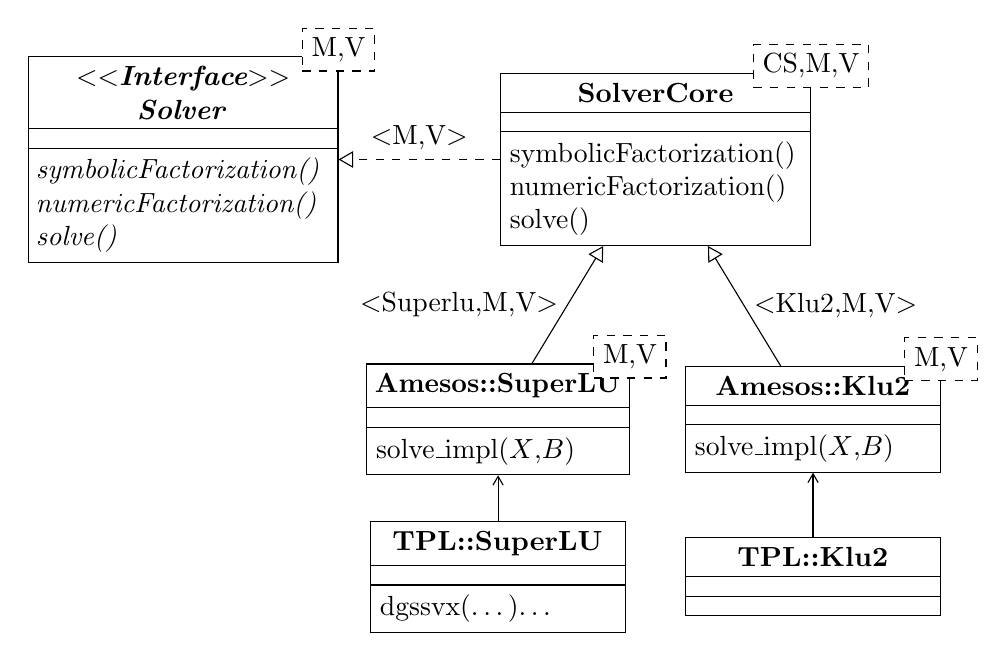
\begin{tikzpicture}
  \myclass[3.7cm]{(6,1.3)}{solvercore}{SolverCore}{CS,M,V}{}{symbolicFactorization()\\numericFactorization()\\solve()}
  \myclass[3.7cm]{($(solvercore) + (-6,0)$)}{solver}{\itshape $<<$Interface$>>$\\Solver}{M,V}{}{\itshape symbolicFactorization()\\numericFactorization()\\solve()}
  \myclass[3.1cm]{(4,-2)}{superlu}{Amesos::SuperLU}{M,V}{}{solve\_impl($X$,$B$)}
  \myclass[3cm]{(4,-4)}{tsuperlu}{TPL::SuperLU}{}{}{dgssvx(\ldots)\ldots}
  \myclass[3cm]{(8,-2)}{klu2}{Amesos::Klu2}{M,V}{}{solve\_impl($X$,$B$)}
  \myclass[3cm]{(8,-4)}{tklu2}{TPL::Klu2}{}{}{}
  
  \draw[implementation] (solvercore) -- node[above] {$<$M,V$>$} (solver);
  \draw[generalization] (superlu) -- node[left] {$<$Superlu,M,V$>$} (solvercore);
  \draw[generalization] (klu2) -- node[right] {$<$Klu2,M,V$>$} (solvercore);
  \draw[association] (tsuperlu) -- (superlu);
  \draw[association] (tklu2) -- (klu2);
  
%\node[rectangle, red, fit=(solver) (tsuperlu) (superlu) (tmumps) (mumps)] {};
\end{tikzpicture}
\end{frame}

\begin{frame}[fragile,shrink,c]
  \frametitle{Internal Design: MatrixAdapter Hierarchy}
%% \begin{verbatim}        
%%                                +---+
%%                 +--------------+ M |
%%                 | MatrixAdapter +--+
%%                 +---------------+        
%%                 | RCP<M> mat_   |     +-------------------------+
%%                 +---------------+     | ...                     |
%%                 | getCrs()  ..........| getGlobalRowCopy(...)   |...
%%                 | getCcs()      |     | ...                     |  .
%%                 +---------------+     +-------------------------+  .
%%              <Derived> ^                                           .
%%                        |           +---------------+               .
%%     +------------------------------+ Abstr,Derived |               .
%%     | AbstractConcreteMatrixAdapter +--------------+               .
%%     +-------------------------------+                              .
%%     | getGlobalRowCopy_impl()       | <.............................
%%     +-------------------------------+                    calls
%%            <super_t,M> ^
%%                        |            +---+
%%              +----------------------+ M |
%%              | ConcreteMatrixAdapter +--+
%%              +-----------------------+
%% \end{verbatim}
\begin{centering}
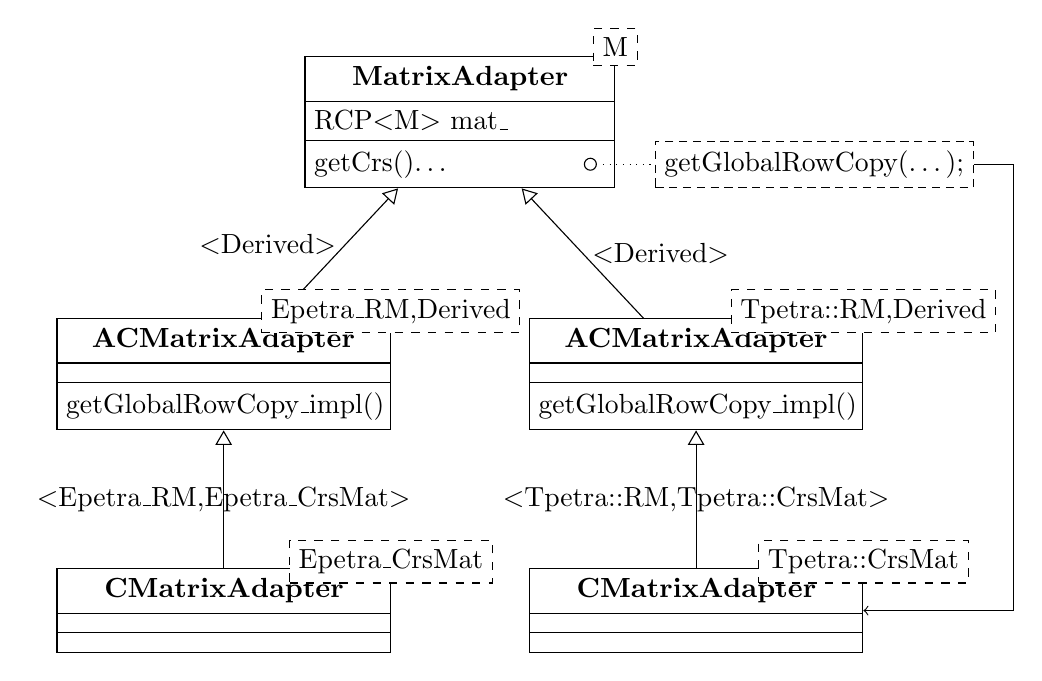
\begin{tikzpicture}
  \myclass[3.7cm]{(0,0)}{matrixadapter}{MatrixAdapter}{M}{RCP$<$M$>$ mat\_}{getCrs()\ldots}
  \path ($(matrixadapter) + (-3,-3.2)$) coordinate(ghost) ;
  \draw[generalization] (ghost) -- node[left,pos=.7]{$<$Derived$>$} (matrixadapter);
  \myclass[4cm]{(ghost)}{acmatadpte}{ACMatrixAdapter}{Epetra\_RM,Derived}{}{getGlobalRowCopy\_impl()}
  \myclass[4cm]{($(matrixadapter) + (3,-3.2)$)}{acmatadptt}{ACMatrixAdapter}{Tpetra::RM,Derived}{}{getGlobalRowCopy\_impl()}
  
  \myclass[4cm]{($(acmatadptt) + (0,-3)$)}{cmatadpttcrs}{CMatrixAdapter}{Tpetra::CrsMat}{}{}
  \myclass[4cm]{($(acmatadpte) + (0,-3)$)}{cmatadptecrs}{CMatrixAdapter}{Epetra\_CrsMat}{}{}

  \draw[generalization] (acmatadptt) -- node[right]{$<$Derived$>$} (matrixadapter);
  \draw[generalization] (cmatadpttcrs) -- node{$<$Tpetra::RM,Tpetra::CrsMat$>$} (acmatadptt);
  \draw[generalization] (cmatadptecrs) -- node{$<$Epetra\_RM,Epetra\_CrsMat$>$} (acmatadpte);

  \node[draw,densely dashed,rectangle,anchor=west] (method) at ($(matrixadapter.third east) + (0.5,0)$) {getGlobalRowCopy(\ldots);} ;

  \draw[dotted,o-] ($(matrixadapter.third east) - (.4,0)$) -- (method);

  \draw[->] (method.east) -- +(0.5,0) |- (cmatadpttcrs);
\end{tikzpicture}
\end{centering}
\end{frame}

\begin{frame}
  \frametitle{Future Work}
  \begin{itemize}
  \item Need better support for pre-ordering: Zoltan2 will provide
    both graph partitoning based and minimum degree based orderings.
  \item Currently we use SuperLU's internal orderings. KLU2 uses the
    orderings from Amesos.
  \item Need to support more solvers and matrix types.
  \end{itemize}
\end{frame}

\end{document}
